\section{YouCook: progettazione}
La struttura dell'applicazione è la seguente
\begin{figure}[H]
    \centering
 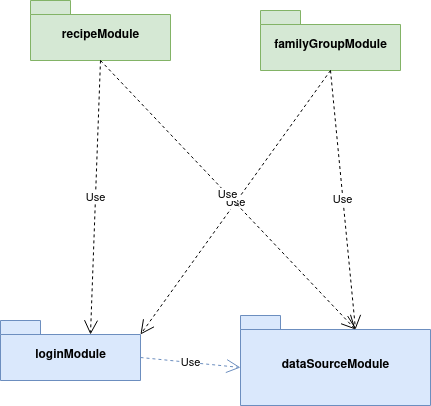
\includegraphics[scale=0.7]{resources/diagramma_package-diagramma_package.drawio.png}
   \caption{Diagramma dei package dell'applicazione}
\end{figure}
L'applicazione è composta da 4 module: i module recipe e familygroup implementano le rispettive funzionalità e sfruttano i servizi offerti dai module login e dataSource per autenticare gli utenti e realizzare la persistenza dei dati. 
\begin{figure}[H]
    \centering
 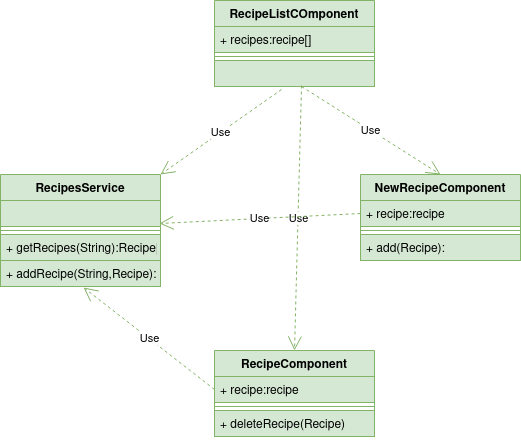
\includegraphics[scale=0.7]{resources/diagramma_package-recipe.drawio.png}
   \caption{Diagramma delle classi pakage recipe}
\end{figure}
 
\begin{figure}[H]
    \centering
 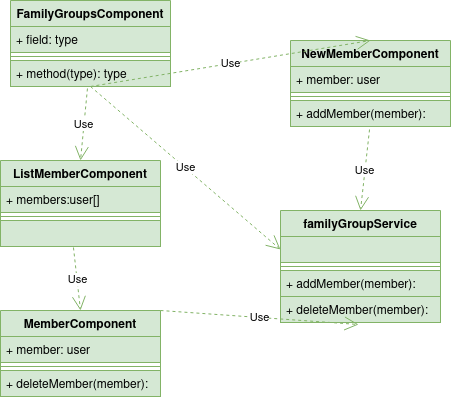
\includegraphics[scale=0.7]{resources/diagramma_package-FamilyGroup.drawio.png}
   \caption{Diagramma delle classi pakage FamilyGroup}
\end{figure}
I componenti dei package Recipe e FamilyGroup sfruttano la strategia di change detection onPush per aggiornare la lista di elementi mostrate nella view e sfruttano i rispettivi Service per interagire con la lista di elementi. Questi ultimi restituiscono a ogni modifica una nuova istanza della lista per attivare il meccanismo  di change detection.
\newline
È stato deciso di delegare la gestione della generazione degli oggetti a un service apposito, cosi da sollevare i componenti dalla necessità di implementare la logica applicativa. In questo modo i componenti possono concentrarsi sulla gestione della interfaccia e in caso si necessiti di modificare la logica con cui vengono gestiti i dati sarà sufficiente agire sul service.
\newpage
\begin{figure}[H]
    \centering
 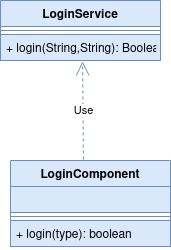
\includegraphics[scale=0.7]{resources/diagramma_package-login.drawio.png}
   \caption{Diagramma delle classi pakage login}
\end{figure}
\begin{figure}[H]
    \centering
 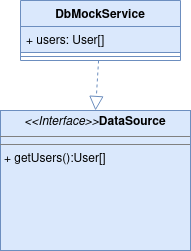
\includegraphics[scale=0.7]{resources/diagramma_package-dataSource.drawio.png}
   \caption{Diagramma delle classi pakage dataSource}
\end{figure}
Il package DataSource sfrutta il pattern strategy per implementare la persistenza verso i data store tramite l'interfaccia DataSource. In questo modo si astrae l'applicazione dalla gestione dello storage dei dati e consentire il recupero dei dati da datastore differenti.
\newline
I package login e datasource mettono ha disposizione una classe service per fornire le funzionalità agli altri componenti.




%- capitolo 1 e capitolo 2 vanno abbastanza bene, mentre il capitolo 3 è deboluccio.
%Riporti anche motivazioni più estese delle scelte fatte, screenshot dell'applicazione realizzata che la aiutino a descriverne le funzionalità. Servirebbero anche dati numerici sulle prestazioni di performance, ma forse a questo punto non ha più il tempo di farle...